% Gemini theme
% https://github.com/anishathalye/gemini

\documentclass[final]{beamer}

% ====================
% Packages
% ====================

\usepackage[T1]{fontenc}
\usepackage{lmodern}
\usepackage[size=custom,width=100,height=72,scale=1.0]{beamerposter}
\usetheme{gemini}
\usecolortheme{gemini}
\usepackage{graphicx}
\usepackage{booktabs}
\usepackage{tikz}
%\usepackage{pgfplots}


\usepackage{copyrightbox}
\makeatletter
\renewcommand{\CRB@setcopyrightfont}%
    {\tiny\color{gray}}
\makeatother
%\usepackage[font=small,skip=0pt]{caption}

\usepackage{caption}
\captionsetup{justification   = raggedright,
              singlelinecheck = false}

% ====================
% Lengths
% ====================

% If you have N columns, choose \sepwidth and \colwidth such that
% (N+1)*\sepwidth + N*\colwidth = \paperwidth
\newlength{\sepwidth}
\newlength{\colwidth}
\setlength{\sepwidth}{0.025\paperwidth}
\setlength{\colwidth}{0.3\paperwidth}

\newcommand{\separatorcolumn}{\begin{column}{\sepwidth}\end{column}}

% ====================
% Title
% ====================

\title{Informal Labour Blues: Effects of COVID-19 and beyond on women belonging to backward castes in India}

\author{Malvya Chintakindi\inst{1} \inst{*}}

\institute[shortinst]{\inst{1} PhD Student \samelineand \inst{*} Advised by: Prof. Lamia Karim}

% ====================
% Footer (optional)
% ====================

\footercontent{
  \href{https://https://anthropology.uoregon.edu}{https://anthropology.uoregon.edu} \hfill
  Department of Anthropology \hfill
  \href{mailto:malvyac@uoregon.edu}{malvyac@uoregon.edu}}
% (can be left out to remove footer)

% ====================
% Logo (optional)
% ====================

% use this to include logos on the left and/or right side of the header:
 \logoright{
\includegraphics[height=7cm]{image-4.png}}
% \logoleft{\includegraphics[height=7cm]{logo2.pdf}}

% ====================
% Body
% ====================

\begin{document}

\begin{frame}[t]
\begin{columns}[t]
\separatorcolumn

\begin{column}{\colwidth}

  \begin{block}{Background}

COVID-19 struck people all over the world, indiscriminately,
altering human living conditions. India was the third worst hit
country in 2020, comprising the largest number of confirmed
cases in Asia. In 2021, India broke world records with its
massive second wave registering highest official daily
infection rates while the unofficial rates are understood to be
soaring. Preliminary data and evidence from several parts of
the world indicate that the incidence of the disease is not
class-neutral and gender-neutral, suggesting that socially
marginalized groups are at higher risk of mortality due to
COVID-19. India’s phased lockdown, imposed in the last week
of March 2020, was among the strictest in the world. With
little to no income, these socially marginalized sections face
challenges to their livelihoods, health, familial and socioeconomic
conditions. The effects of COVID-19 on women
belonging to backward caste communities in India are a case
in point to investigate the multifold effects of the pandemic at
the intersection of gender, class and labour conditions. The
sister states of Andhra Pradesh (AP) and Telangana (TS) in
South India face interstate migration and share business and
information technology partnerships along with several
natural resources, at Hyderabad city. This has aggravated the
burden on infrastructural resources, COVID-19 testing centres
and available hospital beds in Hyderabad, including the
disastrous effect on migrant and non-migrant informal
labourers. Hyderabad is also known to be consistently
spending the nation’s highest on populations that face poor
socio-economic conditions. To fill gaps in understanding the
gravity of the crisis and in the absence of nuanced quantitative
data , anecdotal information is vital to bring to fore the
condition of informal labourers in urban India. This research is
positioned to investigate long term effects of shocks such as
COVID-19 on low income and socio-economically backward
populations in parts of India and other comparable
communities.

\vspace{2cm}

\begin{figure}
\copyrightbox[b]{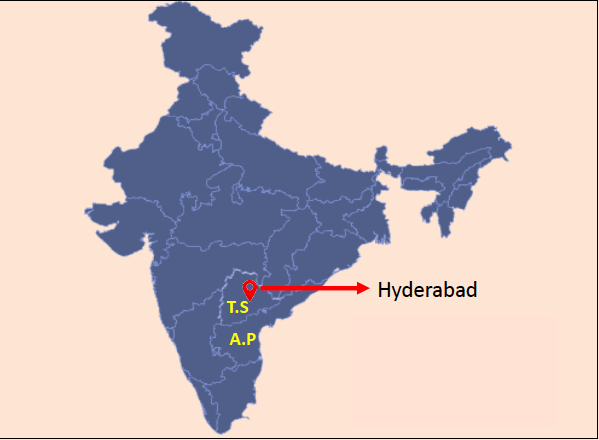
\includegraphics[scale=1.4]{image1.png}}%
                {Map not to scale. For illustration purpose only}
\caption{Map of India with state boundaries only}
\end{figure}
  \end{block}
\end{column}

\separatorcolumn

\begin{column}{\colwidth}

\begin{figure}
\copyrightbox[b]{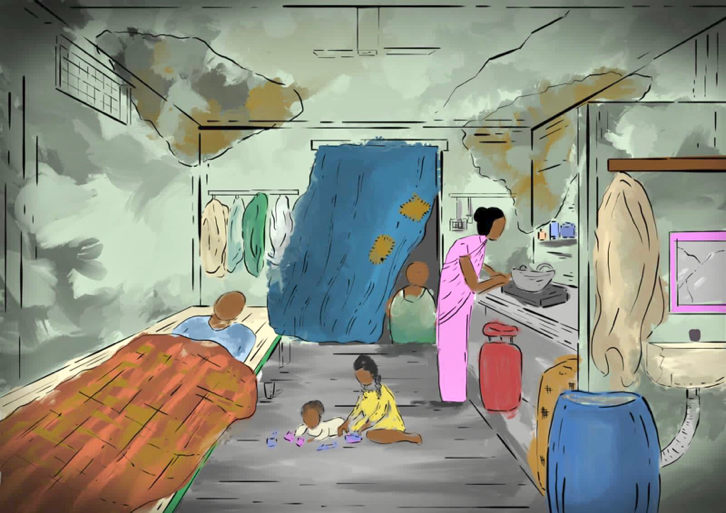
\includegraphics[width=\colwidth]{image-2.png}}%
                  {Illustrator: Niharika}
      \vspace{-1.2cm}  
\caption{Lady in Pink: Engaged in multiple forms of care-taking for her family members
before stepping out for work}
\end{figure}

  \begin{block}{About}

This research encompasses primary field work from September 2020,
leading up to March 2021 in two regions of Hyderabad. Rooted in
grounded theory, the research employs participatory and qualitative
methods such as in-depth interviews, visual aids and participant
observation. Informal semi-structured interviews were conducted with
women from 5 families belonging to backward castes working as
household help and when possible, open ended interviews were
conducted with their children. These women are aged mid 20s-late 50s,
receiving a monthly salary ranging from INR 1000-4000 (\$13.2-\$54) per
household per month. Their children are pursuing education ranging
from middle school to under-graduation. Few of these families are
migrants from AP, whereas TS is the native state of others. Each woman
on average works in three to four households. Some of the women are
educated either until middle school or high school. They juggle a
multitude of responsibilities ranging from their own household chores,
cooking, taking care of the elderly and stepping out to work in
households. The findings include direct quotes from participants.

  \end{block}

  \begin{block}{Findings}

  The lockdown has caused the participants’ job insecurity, with finances
and access to healthcare taking a large hit. Since the lockdown, most
women have been asked to not work as household help by their
employers owing to the fear of spread of the disease and government
restrictions on public mobility.

\end{block}

 \begin{alertblock}{}

‘We have not heard of COVID-19 or
of its spread from government
sources but received some money
and rice grain from our local
government for a couple of
months. Ever since we returned to
the city, we haven’t received
anything’- 35 yrs

  \end{alertblock}


%\end{block}

\end{column}

\separatorcolumn

\begin{column}{\colwidth}

Husbands of these women
primarily work either as
watchmen or as daily wage
labourers. With their husbands
losing their low paying jobs,
the onus of supporting their
households has fallen on women.
\vspace{0.5cm}

The efforts of the government
and civil societies in supporting
informal labourers has been
met with varied outcomes.
Government information
campaigns have not reached
most locations and migrant
families had to travel long
distances by foot to their
hometowns.


  \begin{alertblock}{}

‘We have not heard of COVID-19 or
of its spread from government
sources but received some money
and rice grain from our local
government for a couple of
months. Ever since we returned to
the city, we haven’t received
anything’- 35 yrs

  \end{alertblock}

  These participants’ informal
jobs are now their salvation,
providing a safety net for their
families. They have been highly
stressed for their children’s
education and future. The lack
of technology, internet and
smart mobile phones has been
a huge barrier for their children
to attend online classes.

  \begin{alertblock}{}

‘My eldest girl is going to get
married in December 2020. I
have taken several loans required
for dowry and other wedding
expenses. I don’t know how to
repay and recuperate since my
husband is unemployed. It is all
on me’ - 45 yrs

  \end{alertblock}

  While a couple of participants
reported that lack of income and
loss of jobs meant less alcohol
consumption and less domestic
violence, others mentioned that
nation-wide lockdown induced
irritation and mental stress led to
their husbands’ higher alcohol
consumption and desperate
alcohol purchase with savings. All
participants felt the need for
social protection and welfare
assurance measures since there
is no uniform agency that
addresses the grievances of
informal labour. The participants
and their networks feel a sense of
abandonment and isolation. They
stated to have been incapable in
developing functional coping
mechanisms in their day-to-day
stressful situations. There
is moderate trust on vaccines but
due to the wide shortage of
essential supplies and
medication, they feel dejected
and uncertain about access.

  \begin{alertblock}{}

‘We cannot kill ourselves by
staying stuck at home without
income. I do not care about my
health and safety anymore. I
need to work so I can put food
on our plates. Whatever will
happen, will happen’ - 36 yrs
  \end{alertblock}
 

  \begin{block}{Next Steps}

The research will incorporate a
larger sample and further
explore questions surrounding
gendered effects of the
pandemic on informal labour
and unravel multiplicities of
vulnerabilities. The research will
turn to marginalized
communities in other parts of
India to deeply understand their
conditions owing to the
pandemic and the overall
impact on their status. There
will be an emphasised focus on
women empowerment, gender
equality, development
aspirations and health
outcomes.
  \end{block}

  \begin{block}{References}

    \nocite{*}
    \footnotesize{\bibliographystyle{plain}\bibliography{poster}}

  \end{block}

\end{column}
\separatorcolumn

\end{columns}
\end{frame}

\end{document}
